\documentclass[10 pt,usenames,dvipsnames, oneside]{article}
\usepackage{../../../modelo-ensino-medio}



\begin{document}

\begin{center}
  \begin{minipage}[l]{3cm}

\includegraphics[width=2cm]{logo}    
\end{minipage}\hfill
\begin{minipage}[r]{.8\textwidth}
 {\Large \scshape Atividade: Estudando o sinal de uma função afim usando o GeoGebra}  
\end{minipage}
\end{center}
\vspace{.2cm}

\ifdefined\prof
%Habilidades da BNCC
% \begin{objetivos}
% \item 
% \end{objetivos}

%Caixa do Para o Professor
\begin{goals}
%Objetivos específicos
\begin{enumerate}
\item Estudar a variação do sinal de uma função afim. 
\item Estabelecer condições para que a função afim seja crescente ou decrescente.
\item Compreender o significado geométrico do sinal de uma função afim.
\end{enumerate}

\tcblower

%Orientações e sugestões
Professor, essa é uma construção que contribuirá para que o aluno compreenda o significado do estudo da variação do sinal de uma função. É muito comum que o aluno confunda o sinal de $x$ com o sinal de $y$. Por essa razão, a construção do segmento orientado vai auxiliar a que ele perceba que, conforme $x$ cresce, a função tem seu sinal variando de acordo com a localização de sua raiz, de negativo para positivo, se a função for crescente, e de positivo para negativo, se a função for decrescente. Certifique-se de que o aluno sempre movimente o ponto livre construído no eixo $Ox$ para a esquerda ao máximo possível para iniciar sua observação. Você pode ainda sugerir que o estudante habilite o rastro do segmento orientado (vetor) construído, de forma que ele visualizará regiões sob/sobre o eixo dos $x$, enfatizando a variação do sinal. Veja como ficaria habilitando o rastro.
\end{goals}

\bigskip
\begin{center}
{\large \scshape Atividade}
\end{center}
\fi

Vamos fazer uma construção usando o GeoGebra. Siga os seguintes passos:

1-	Abra a janela gráfica e escreva $y=a(x-p)^2+q$ no campo de entrada e tecle ENTER;

\begin{figure}[H]
\centering
\noindent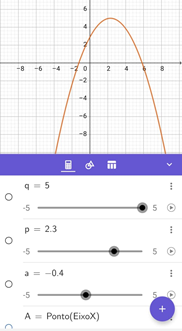
\includegraphics[width=150bp]{inequacao4}
\end{figure}

Observe que o GeoGebra denominou por $f$ à função que associa $x$ e $y$ por meio da lei algébrica $y=a(x-p)^2+q$ e gerou, automaticamente, três controles deslizantes para os valores de $a$, $p$ e $q$, variando de $-5$ a $5$. Movimente os controles deslizantes e verifique o que ocorre com a função. Quais os significados geométricos, na parábola, dos parâmetros $a$, $p$ e $q$?

\begin{figure}[H]
\centering
\noindent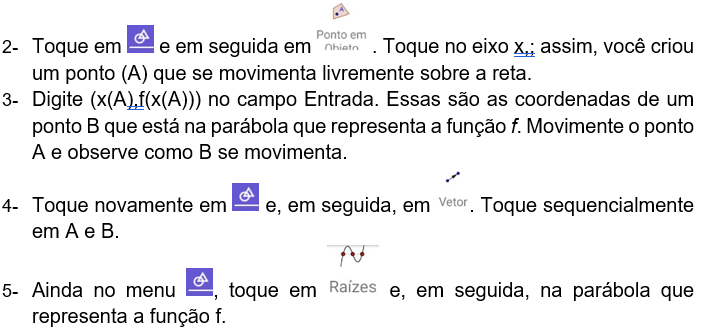
\includegraphics[width=400bp]{icones2}
\end{figure}
Agora vamos explorar um pouco a sua construção?

\begin{enumerate}
\item{} Ajuste o controle deslizante $a$ para um valor maior que zero. Como está a concavidade da função $f$?

\item {} Mantenha o controle deslizante $a$ fixo com o valor usado no item \titem{a)}. Arraste o ponto $A$ para o canto mais esquerdo do eixo $x$ e ajuste os controles $p$ e $q$ de forma que tenhamos duas raízes para a função $f$. Qual o sinal do discriminante $\Delta$?

\item{}	
Movimente lentamente o ponto $A$ no sentido positivo do eixo $x$. O que você observa sobre o vetor $\overrightarrow{AB}$? Descreva a posição desse vetor de acordo com as raízes da função $f$.
\end{enumerate}

\ifdefined\prof
\begin{solucao}

\begin{enumerate}
\item Crescente.
\item Conforme o ponto $A$ avança do negativo para o positivo, o vetor  muda sua orientação de "apontando para baixo" para "apontando para cima", acompanhando o sinal da função (quando a função é negativa, ele aponta para baixo, quando ela é positiva, ele aponta para cima).
\item Decrescente.
\item Conforme o ponto $A$ avança do negativo para o positivo, o vetor  muda sua orientação de "apontando para cima" para "apontando para baixo", acompanhando o sinal da função.
\item o vetor $\overrightarrow{AB}$ alterna o seu sentido de cima para baixo exatamente quando o ponto $A$ se encontra sobre o zero da função afim.
\end{enumerate}

\end{solucao}
\fi

\end{document}